\documentclass{article}\usepackage[]{graphicx}\usepackage[]{color}
%% maxwidth is the original width if it is less than linewidth
%% otherwise use linewidth (to make sure the graphics do not exceed the margin)
\makeatletter
\def\maxwidth{ %
  \ifdim\Gin@nat@width>\linewidth
    \linewidth
  \else
    \Gin@nat@width
  \fi
}
\makeatother

\definecolor{fgcolor}{rgb}{0.345, 0.345, 0.345}
\newcommand{\hlnum}[1]{\textcolor[rgb]{0.686,0.059,0.569}{#1}}%
\newcommand{\hlstr}[1]{\textcolor[rgb]{0.192,0.494,0.8}{#1}}%
\newcommand{\hlcom}[1]{\textcolor[rgb]{0.678,0.584,0.686}{\textit{#1}}}%
\newcommand{\hlopt}[1]{\textcolor[rgb]{0,0,0}{#1}}%
\newcommand{\hlstd}[1]{\textcolor[rgb]{0.345,0.345,0.345}{#1}}%
\newcommand{\hlkwa}[1]{\textcolor[rgb]{0.161,0.373,0.58}{\textbf{#1}}}%
\newcommand{\hlkwb}[1]{\textcolor[rgb]{0.69,0.353,0.396}{#1}}%
\newcommand{\hlkwc}[1]{\textcolor[rgb]{0.333,0.667,0.333}{#1}}%
\newcommand{\hlkwd}[1]{\textcolor[rgb]{0.737,0.353,0.396}{\textbf{#1}}}%

\usepackage{framed}
\makeatletter
\newenvironment{kframe}{%
 \def\at@end@of@kframe{}%
 \ifinner\ifhmode%
  \def\at@end@of@kframe{\end{minipage}}%
  \begin{minipage}{\columnwidth}%
 \fi\fi%
 \def\FrameCommand##1{\hskip\@totalleftmargin \hskip-\fboxsep
 \colorbox{shadecolor}{##1}\hskip-\fboxsep
     % There is no \\@totalrightmargin, so:
     \hskip-\linewidth \hskip-\@totalleftmargin \hskip\columnwidth}%
 \MakeFramed {\advance\hsize-\width
   \@totalleftmargin\z@ \linewidth\hsize
   \@setminipage}}%
 {\par\unskip\endMakeFramed%
 \at@end@of@kframe}
\makeatother

\definecolor{shadecolor}{rgb}{.97, .97, .97}
\definecolor{messagecolor}{rgb}{0, 0, 0}
\definecolor{warningcolor}{rgb}{1, 0, 1}
\definecolor{errorcolor}{rgb}{1, 0, 0}
\newenvironment{knitrout}{}{} % an empty environment to be redefined in TeX

\usepackage{alltt}

\usepackage{comment}
\usepackage[english]{isodate}

\usepackage{graphicx}
\usepackage{siunitx}
\usepackage{paracol}
\usepackage{amsmath}
\usepackage{ amssymb }
\usepackage[utf8]{inputenc}
\usepackage[bookmarks=true]{hyperref}
\usepackage{bookmark}

\usepackage{mathtools,xparse}

\DeclarePairedDelimiter{\abs}{\lvert}{\rvert}
\DeclarePairedDelimiter{\norm}{\lVert}{\rVert}

\newcommand{\E}{\mathrm{E}}
\newcommand{\Var}{\mathrm{Var}}
\newcommand{\Cov}{\mathrm{Cov}}
\IfFileExists{upquote.sty}{\usepackage{upquote}}{}
\begin{document}

	\begin{titlepage}
		\begin{center}
			\vspace*{1cm}
			\textbf{Math 423}\\
			\text{Linear Regression}\\
			\vspace{0.5cm}
			Homework I
			
			\vspace{1.5cm}
			
			\textbf{Frédéric Boileau}\\
			\vspace{2cm}
			Prof. 
			David A. Stephens
			\vfill
			\today
			\thispagestyle{empty}
		\end{center}
	\end{titlepage}
	
\section{Data Analysis}

\begin{knitrout}
\definecolor{shadecolor}{rgb}{0.969, 0.969, 0.969}\color{fgcolor}\begin{kframe}
\begin{alltt}
\hlcom{#Read in data set 1}
\hlkwd{library}\hlstd{(lmtest)}
\end{alltt}


{\ttfamily\noindent\color{warningcolor}{\#\# Warning: package 'lmtest' was built under R version 3.3.1}}

{\ttfamily\noindent\itshape\color{messagecolor}{\#\# Loading required package: zoo}}

{\ttfamily\noindent\color{warningcolor}{\#\# Warning: package 'zoo' was built under R version 3.3.1}}

{\ttfamily\noindent\itshape\color{messagecolor}{\#\# \\\#\# Attaching package: 'zoo'}}

{\ttfamily\noindent\itshape\color{messagecolor}{\#\# The following objects are masked from 'package:base':\\\#\# \\\#\#\ \ \ \  as.Date, as.Date.numeric}}\begin{alltt}
\hlstd{file1}\hlkwb{<-}\hlstr{"http://www.math.mcgill.ca/dstephens/Regression/Data/a1-1.txt"}
\hlstd{data1}\hlkwb{<-}\hlkwd{read.table}\hlstd{(file1,}\hlkwc{header}\hlstd{=}\hlnum{TRUE}\hlstd{)}
\hlstd{x1}\hlkwb{<-}\hlstd{data1}\hlopt{$}\hlstd{x}
\hlstd{y1}\hlkwb{<-}\hlstd{data1}\hlopt{$}\hlstd{y}
\hlstd{fit.RP1}\hlkwb{<-}\hlkwd{lm}\hlstd{(y1}\hlopt{~}\hlstd{x1)}
\hlstd{beta0_1} \hlkwb{=} \hlstd{fit.RP1}\hlopt{$}\hlstd{coefficients[}\hlnum{1}\hlstd{]}
\hlstd{beta1_1} \hlkwb{=} \hlstd{fit.RP1}\hlopt{$}\hlstd{coefficients[}\hlnum{2}\hlstd{]}
\hlstd{res1} \hlkwb{=} \hlkwd{residuals}\hlstd{(fit.RP1)}

\hlstd{file2}\hlkwb{<-}\hlstr{"http://www.math.mcgill.ca/dstephens/Regression/Data/a1-2.txt"}
\hlstd{data2}\hlkwb{<-}\hlkwd{read.table}\hlstd{(file2,}\hlkwc{header}\hlstd{=}\hlnum{TRUE}\hlstd{)}
\hlstd{x2}\hlkwb{<-}\hlstd{data2}\hlopt{$}\hlstd{x}
\hlstd{y2}\hlkwb{<-}\hlstd{data2}\hlopt{$}\hlstd{y}
\hlstd{fit.RP2}\hlkwb{<-}\hlkwd{lm}\hlstd{(y2}\hlopt{~}\hlstd{x2)}
\hlstd{beta0_2} \hlkwb{=} \hlstd{fit.RP2}\hlopt{$}\hlstd{coefficients[}\hlnum{1}\hlstd{]}
\hlstd{beta1_2} \hlkwb{=} \hlstd{fit.RP2}\hlopt{$}\hlstd{coefficients[}\hlnum{2}\hlstd{]}
\hlstd{res2} \hlkwb{=} \hlkwd{residuals}\hlstd{(fit.RP2)}

\hlstd{file3}\hlkwb{<-}\hlstr{"http://www.math.mcgill.ca/dstephens/Regression/Data/a1-3.txt"}
\hlstd{data3}\hlkwb{<-}\hlkwd{read.table}\hlstd{(file3,}\hlkwc{header}\hlstd{=}\hlnum{TRUE}\hlstd{)}
\hlstd{x3}\hlkwb{<-}\hlstd{data3}\hlopt{$}\hlstd{x}
\hlstd{y3}\hlkwb{<-}\hlstd{data3}\hlopt{$}\hlstd{y}
\hlstd{fit.RP3}\hlkwb{<-}\hlkwd{lm}\hlstd{(y3}\hlopt{~}\hlstd{x3)}
\hlstd{beta0_3} \hlkwb{=} \hlstd{fit.RP3}\hlopt{$}\hlstd{coefficients[}\hlnum{1}\hlstd{]}
\hlstd{beta1_3} \hlkwb{=} \hlstd{fit.RP3}\hlopt{$}\hlstd{coefficients[}\hlnum{2}\hlstd{]}
\hlstd{res3} \hlkwb{=} \hlkwd{residuals}\hlstd{(fit.RP3)}
\end{alltt}
\end{kframe}
\end{knitrout}



So we have the parameters $\beta_0 = $ $0.0267655$ and $\beta_1 = 1.7251209$ from the linear regression. We plot the data with the line of best fit superimposed
\begin{knitrout}
\definecolor{shadecolor}{rgb}{0.969, 0.969, 0.969}\color{fgcolor}\begin{kframe}
\begin{alltt}
\hlkwd{plot}\hlstd{(x1,y1)}
\hlkwd{abline}\hlstd{(beta0_1, beta1_1)}
\end{alltt}
\end{kframe}
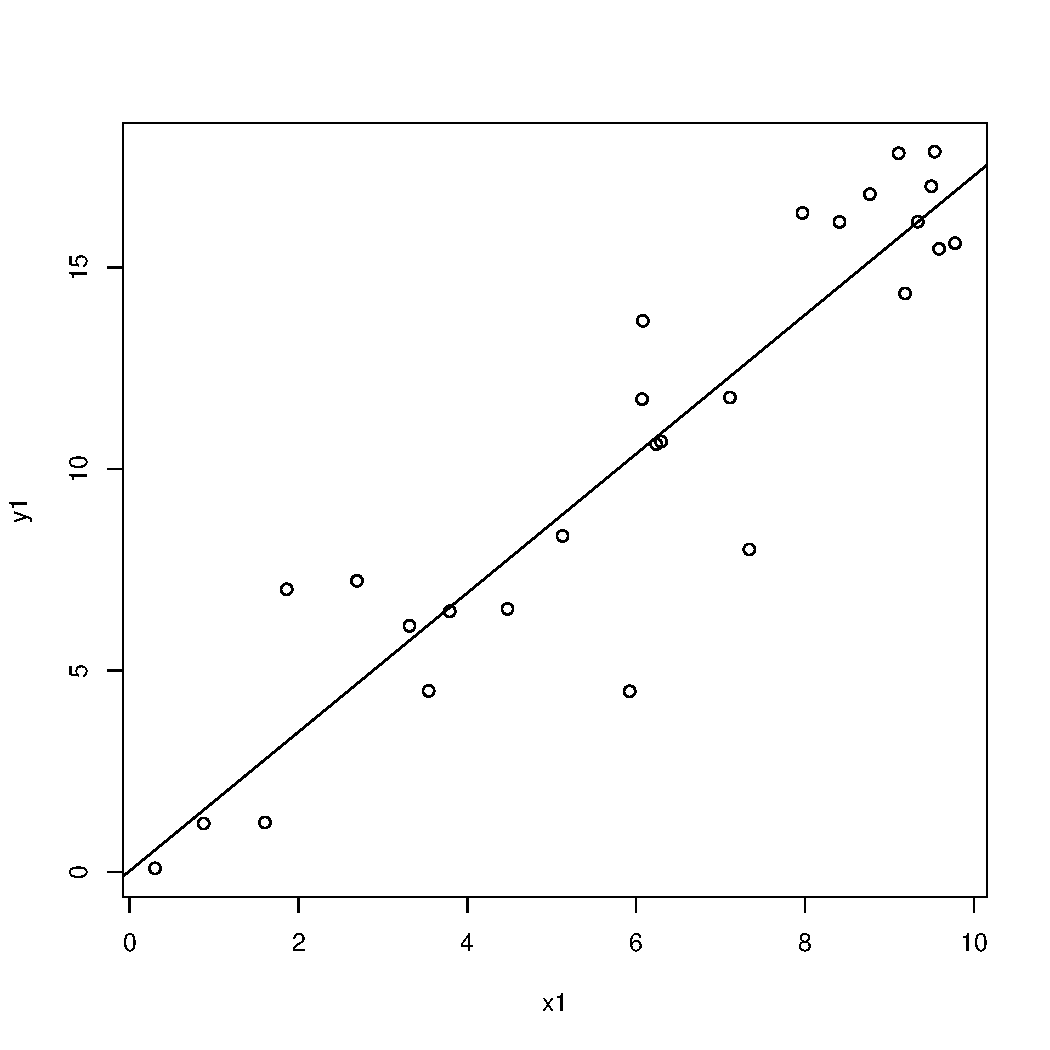
\includegraphics[width=\maxwidth]{figure/unnamed-chunk-2-1} 

\end{knitrout}


\clearpage


\begin{figure}[htbp]
\begin{knitrout}
\definecolor{shadecolor}{rgb}{0.969, 0.969, 0.969}\color{fgcolor}\begin{kframe}
\begin{alltt}
\hlkwd{plot}\hlstd{(x1,res1)}
\end{alltt}
\end{kframe}
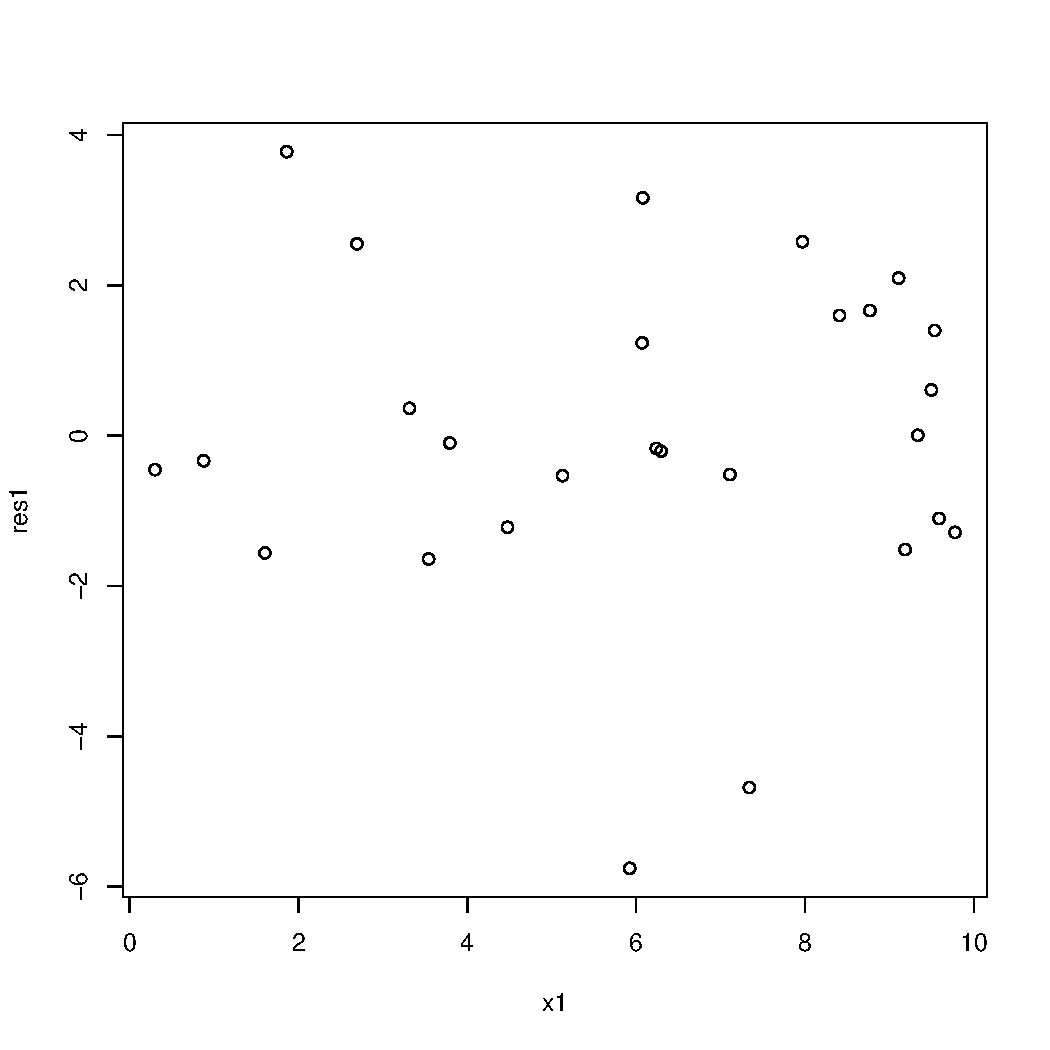
\includegraphics[width=\maxwidth]{figure/unnamed-chunk-3-1} 
\begin{kframe}\begin{alltt}
\hlkwd{mean}\hlstd{(res1)}
\end{alltt}
\begin{verbatim}
## [1] 2.664728e-17
\end{verbatim}
\end{kframe}
\end{knitrout}
\end{figure}
The residual plot seems to display adequate features although hard to tell graphically because of there is not that much data. The mean seemsto be above zero by quick graphicall inspection but is actually virtually null. The variance seems constant. We conclude the linear model used is adequate.



\clearpage

So we have the parameters $\beta_0 = $ $10.6608534$ and $\beta_1 = 7.0379523$ from the linear regression. We plot the data with the line of best fit superimposed
\begin{knitrout}
\definecolor{shadecolor}{rgb}{0.969, 0.969, 0.969}\color{fgcolor}\begin{kframe}
\begin{alltt}
\hlkwd{plot}\hlstd{(x2,y2)}
\hlkwd{abline}\hlstd{(beta0_2, beta1_2)}
\end{alltt}
\end{kframe}
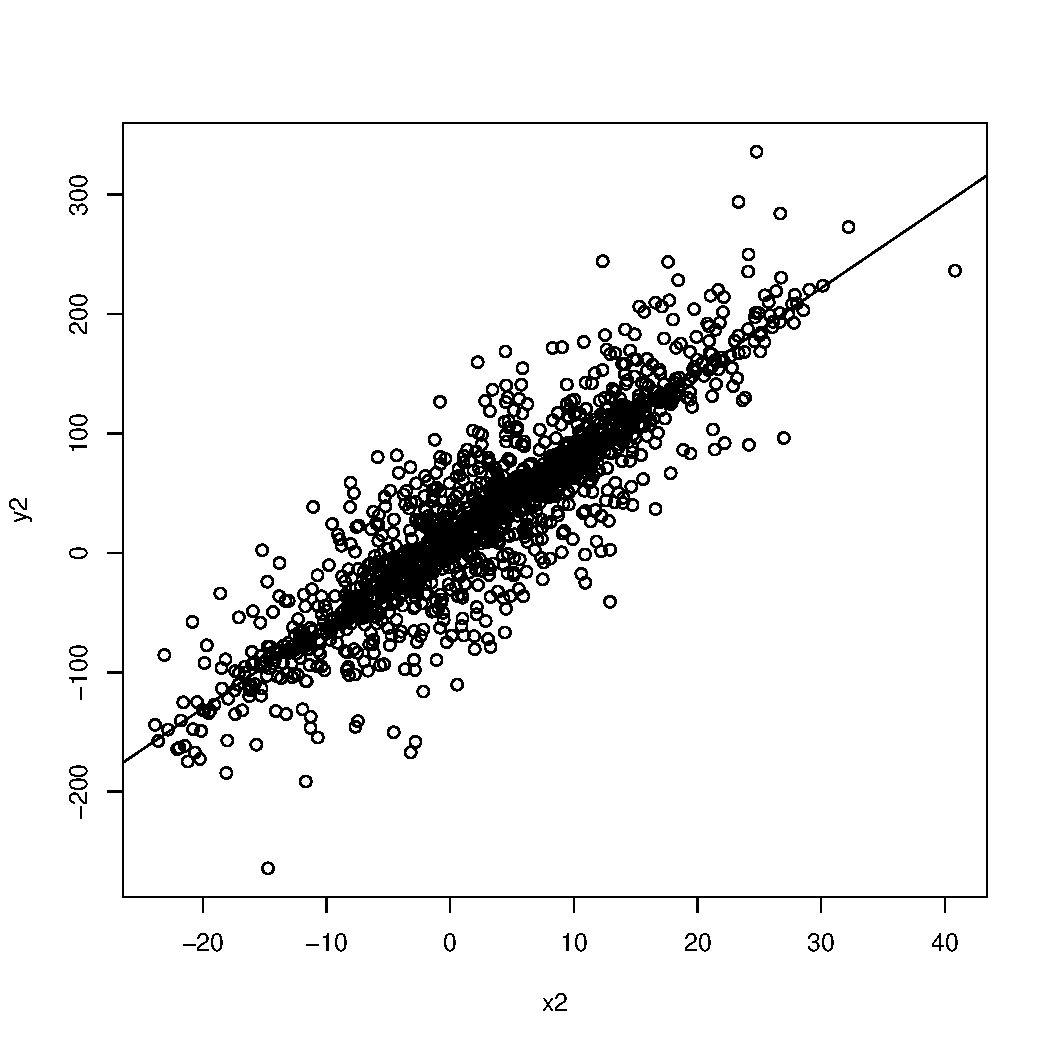
\includegraphics[width=\maxwidth]{figure/unnamed-chunk-4-1} 

\end{knitrout}


\clearpage


\begin{figure}[htbp]
\begin{knitrout}
\definecolor{shadecolor}{rgb}{0.969, 0.969, 0.969}\color{fgcolor}\begin{kframe}
\begin{alltt}
\hlkwd{plot}\hlstd{(x2,res2)}
\end{alltt}
\end{kframe}
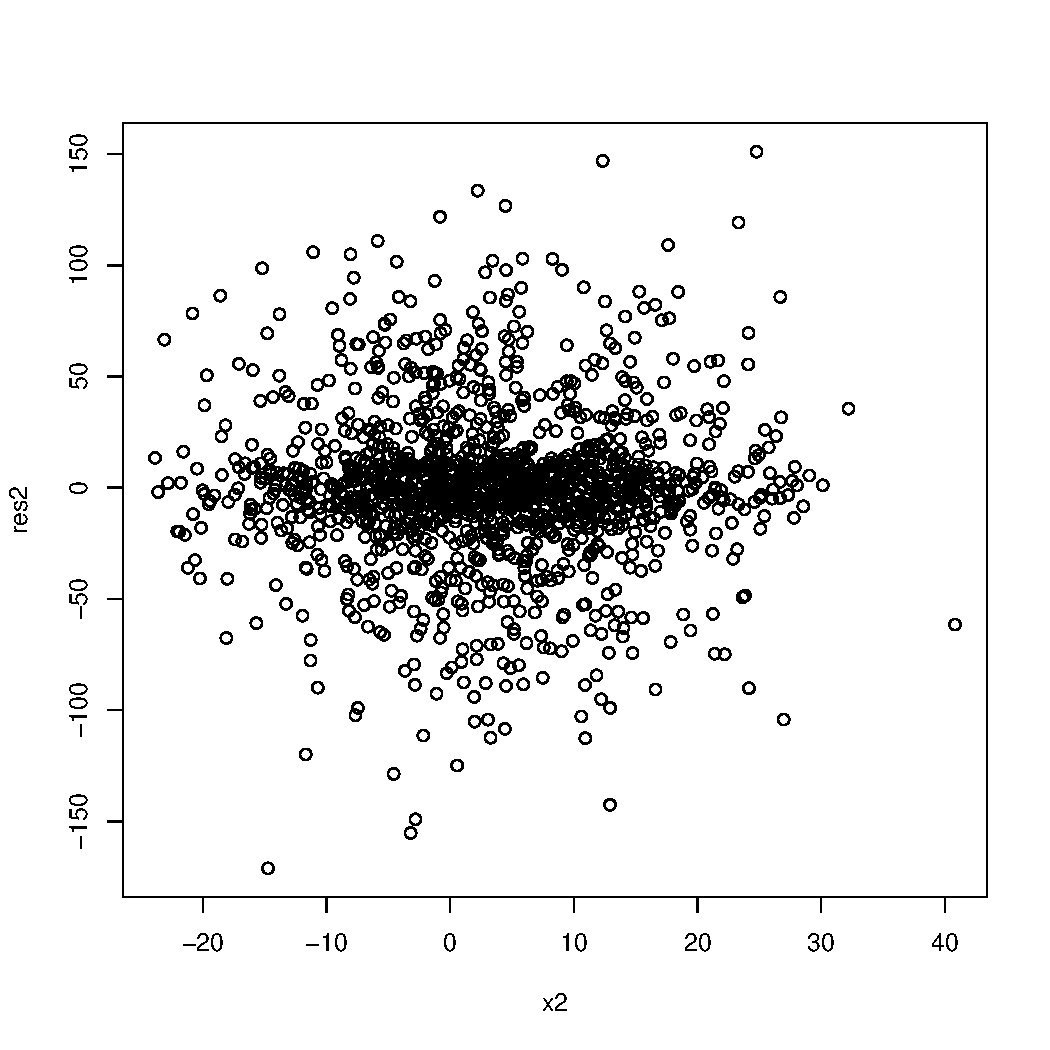
\includegraphics[width=\maxwidth]{figure/unnamed-chunk-5-1} 
\begin{kframe}\begin{alltt}
\hlkwd{mean}\hlstd{(res2)}
\end{alltt}
\begin{verbatim}
## [1] 7.303642e-16
\end{verbatim}
\end{kframe}
\end{knitrout}
\end{figure}
We now plot the residuals next to the corresponding xs. The model seems adequate as the residuals are heavily concentrated around the zero line. The computed mean is again virtually zero (7.30e-16). As for the variance it could seem as if the variance changes but we are careful to notice the distribution of the x's doesn't seem uniform and could explain this graphical impression. 

\clearpage
\begin{knitrout}
\definecolor{shadecolor}{rgb}{0.969, 0.969, 0.969}\color{fgcolor}\begin{kframe}
\begin{alltt}
\hlkwd{boxplot}\hlstd{(res2[}\hlnum{1}\hlopt{:}\hlnum{150}\hlstd{],res2[}\hlnum{151}\hlopt{:}\hlnum{301}\hlstd{],res2[}\hlnum{302}\hlopt{:}\hlnum{452}\hlstd{],res2[}\hlnum{453}\hlopt{:}\hlnum{603}\hlstd{],}
        \hlstd{res2[}\hlnum{604}\hlopt{:}\hlnum{754}\hlstd{],res2[}\hlnum{755}\hlopt{:}\hlnum{900}\hlstd{],res2[}\hlnum{901}\hlopt{:}\hlnum{1051}\hlstd{],res2[}\hlnum{1052}\hlopt{:}\hlnum{1202}\hlstd{],}
        \hlstd{res2[}\hlnum{1203}\hlopt{:}\hlnum{1353}\hlstd{],res2[}\hlnum{1354}\hlopt{:}\hlnum{1445}\hlstd{])}
\end{alltt}
\end{kframe}
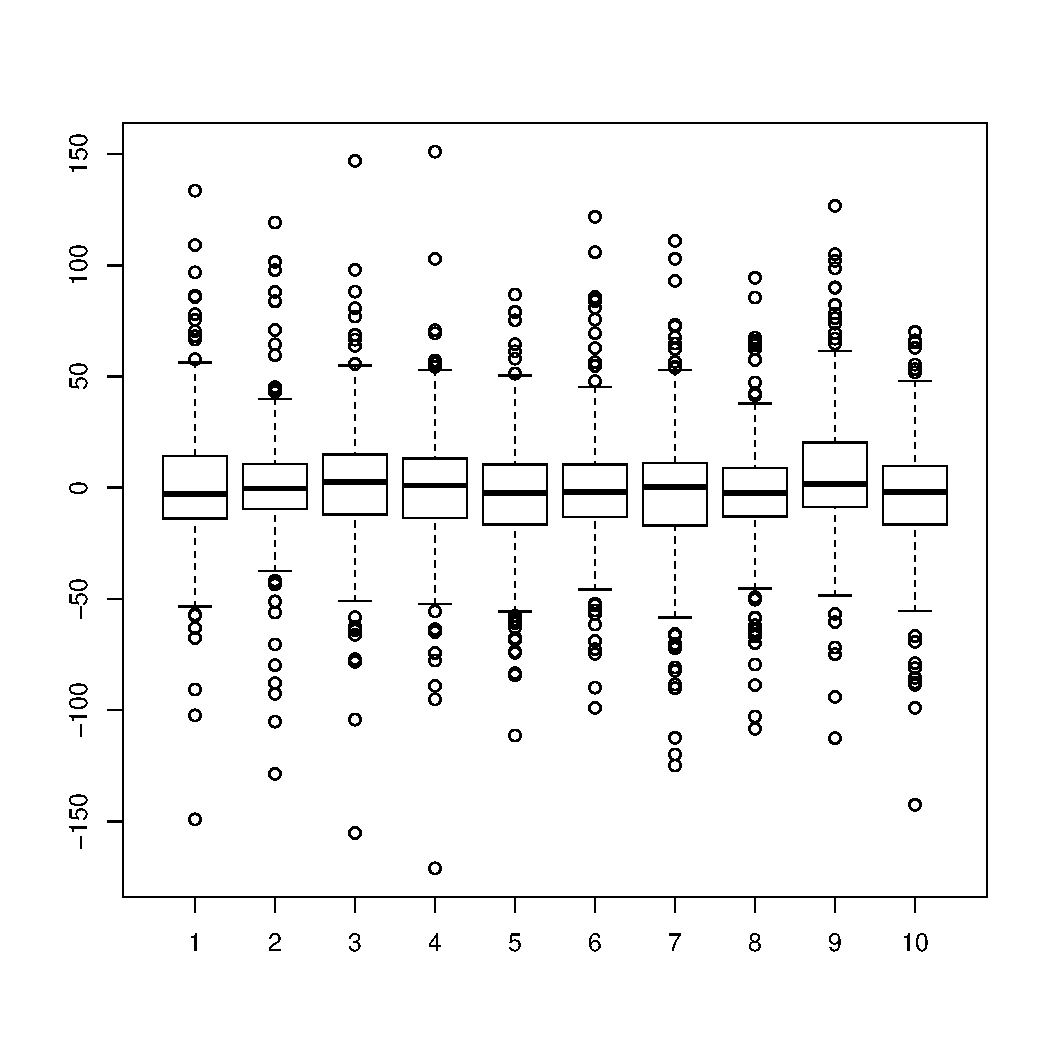
\includegraphics[width=\maxwidth]{figure/unnamed-chunk-6-1} 

\end{knitrout}

The boxplot confirms there is no obvious change in the variance of the residuals. The straight line model we have chosen is therefore appropriate.

\clearpage



So we have the parameters $\beta_0 = $ $0.2403328$ and $\beta_1 = 0.3267628$ from the linear regression. We plot the data with the line of best fit superimposed
\begin{knitrout}
\definecolor{shadecolor}{rgb}{0.969, 0.969, 0.969}\color{fgcolor}\begin{kframe}
\begin{alltt}
\hlkwd{plot}\hlstd{(x3,y3)}
\hlkwd{abline}\hlstd{(beta0_3, beta1_3)}
\end{alltt}
\end{kframe}
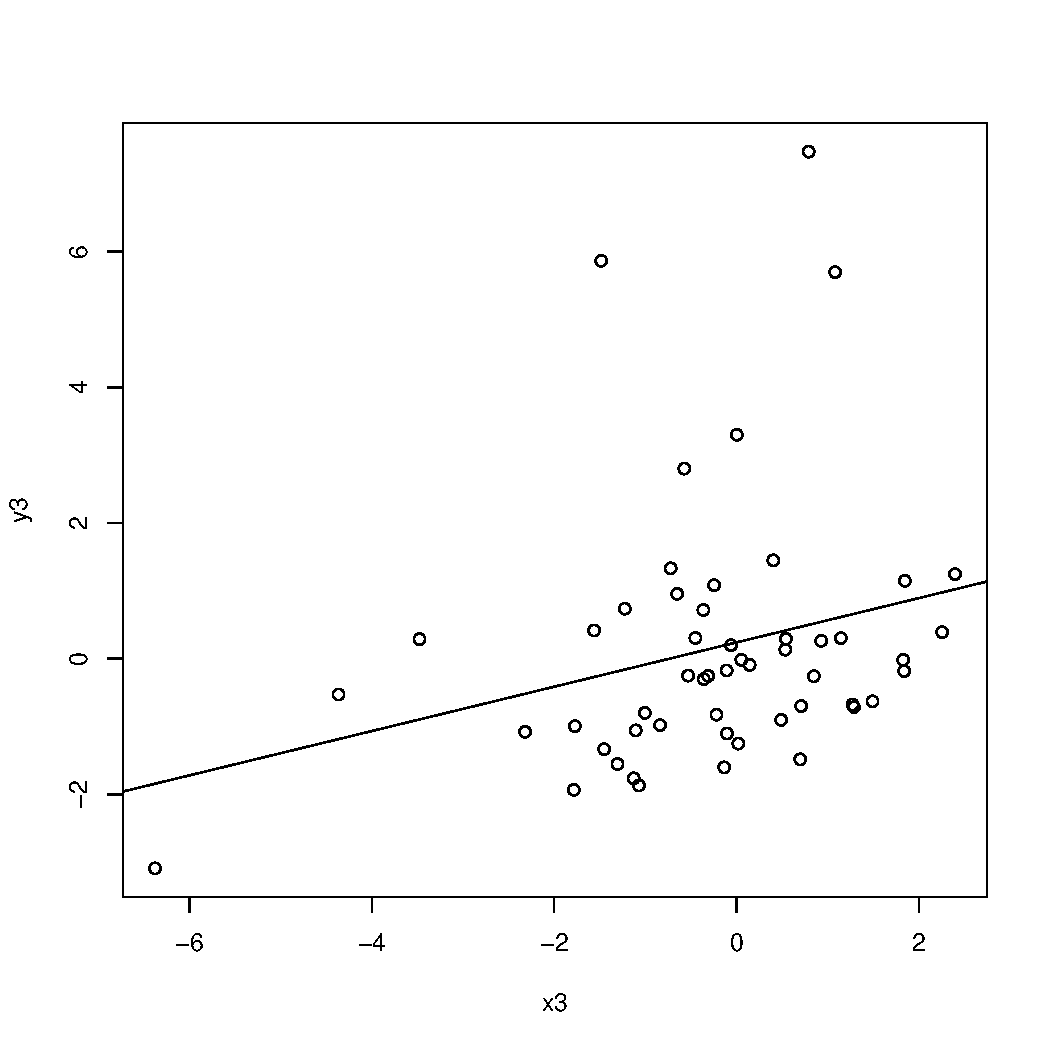
\includegraphics[width=\maxwidth]{figure/unnamed-chunk-7-1} 

\end{knitrout}


\clearpage


\begin{figure}[htbp]
\begin{knitrout}
\definecolor{shadecolor}{rgb}{0.969, 0.969, 0.969}\color{fgcolor}\begin{kframe}
\begin{alltt}
\hlkwd{plot}\hlstd{(x3,res3)}
\end{alltt}
\end{kframe}
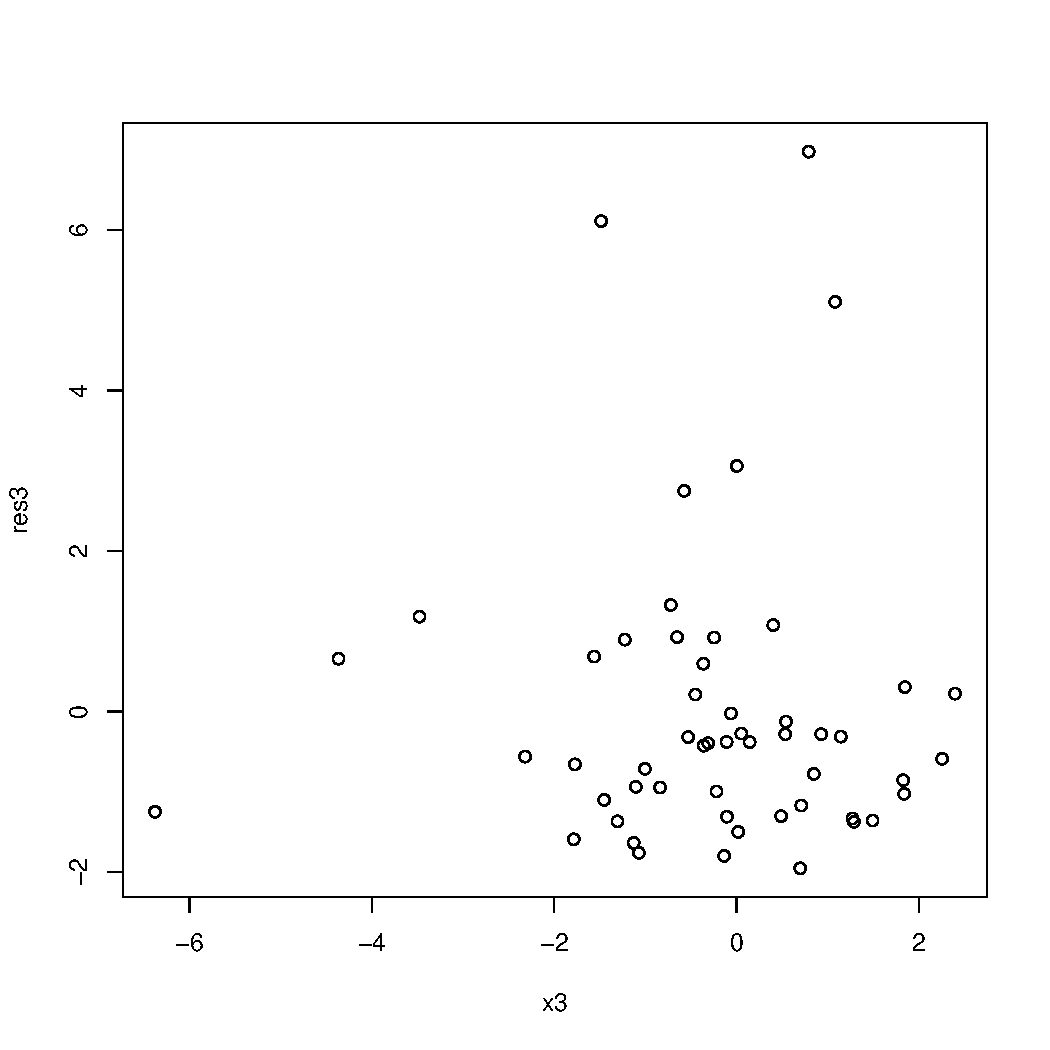
\includegraphics[width=\maxwidth]{figure/unnamed-chunk-8-1} 
\begin{kframe}\begin{alltt}
\hlkwd{mean}\hlstd{(res3)}
\end{alltt}
\begin{verbatim}
## [1] -4.399815e-17
\end{verbatim}
\end{kframe}
\end{knitrout}
\end{figure}
We now plot the residuals next to the corresponding xs. The mean of the residuals is again virtually zero eventhough graphically it seems it could be otherwise. Once again the data in the x's isn't evenly distributed and so is hard to analyze graphically. Even the box plot does not reveal much. Nothing contradicts the model specifically but it looks as if more data would be needed to use it with confidence. 

\clearpage

\begin{knitrout}
\definecolor{shadecolor}{rgb}{0.969, 0.969, 0.969}\color{fgcolor}\begin{kframe}
\begin{alltt}
\hlkwd{boxplot}\hlstd{(res3[}\hlnum{1}\hlopt{:}\hlnum{10}\hlstd{],res3[}\hlnum{11}\hlopt{:}\hlnum{20}\hlstd{],res3[}\hlnum{21}\hlopt{:}\hlnum{30}\hlstd{],res3[}\hlnum{31}\hlopt{:}\hlnum{40}\hlstd{],res3[}\hlnum{40}\hlopt{:}\hlnum{53}\hlstd{])}
\end{alltt}
\end{kframe}
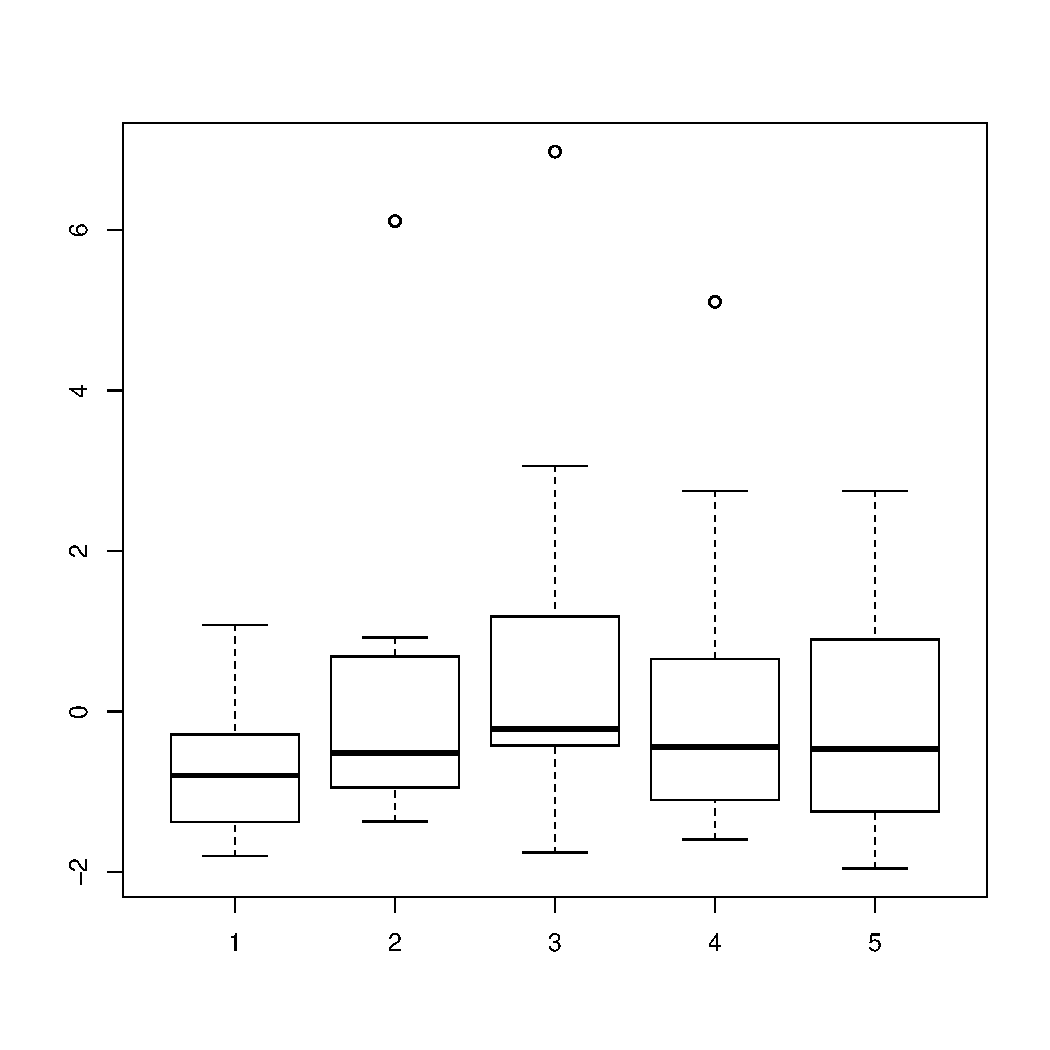
\includegraphics[width=\maxwidth]{figure/unnamed-chunk-9-1} 

\end{knitrout}


\section{Theoretical demonstrations}
\subsection{Location Shift}

	\begin{align*}
		S_{xx} ^* &= \sum_{i=1}^{n}\left[(x_i - m) - (\frac{1}{n}\sum_{i=1}^{n} (x_i- m)) \right]^2  \\
		&= \sum_{i=1}^{n}((x_i - m) - (\bar{x} - m))^2\\
		&= \sum_{i=1}^{n}(x_i -\bar{x})^2 \\
		&= S_{xx}
	\end{align*}
	
	\begin{align*}
		S_{xy}^* &= \sum_{i=1}^{n}y_i\left[(x_i - m) - (\frac{1}{n}\sum_{i=1}^{n} (x_i- m)) \right] \\
		&= \sum_{i=1}^{n} y_i(x_i - \bar{x})\\
		&= S_{xy}
	\end{align*}
 
	
	\begin{align*}
		\hat{\beta}_1^* = \frac{S_{xy}^*}{S_{xx}^*} = \hat\beta_1 \quad \hat\beta_0^* = \bar{y} - \hat\beta_1(\bar x - m)
	\end{align*}
	
		
	As for the properties, since $\hat\beta_1$ doesn't change with scaling it has the same as the ones for the original estimator, namely it is unbiased and we have variance of $\frac{\sigma^2}{S_{xx}}$.
	
	\begin{align*}
		E(\hat\beta_0 ^*) &= E(\bar y - \hat\beta_1 (\bar x - m))\\
		&= E(\bar y) - \beta_1(\bar x - m )\\
		&= \beta_0 + \beta_1 \bar x  - \beta_1\bar x - \beta _1 m\\
		&= \beta_0 - \beta_1 m\\[2ex]
		\Var (\hat \beta_0^* ) &=  \Var(\bar y - \hat \beta_1(\bar x -m))\\
		&= \Var (\hat y)  +(\bar x - m)^2 \Var(\hat{\beta_1}) - 2(\bar x - m)\Cov (\bar y, \hat\beta_1)\\
		&= \sigma ^2\left(\frac{1}{n}+ \frac{(\bar x - m)^2}{S_{xx}}\right)
	\end{align*}
	
\clearpage
	
\subsection{Scaling}

	\begin{align*}
	S_{xx} ^* &= \sum_{i=1}^{n}(l(x_i -\bar{x}))^2 \\[2ex]
	&= l^2 S_{xx}
	\end{align*}
		
	\begin{align*}
	S_{xy}^* &= \sum_{i=1}^{n} y_i(l(x_i - \bar{x}))\\[2ex]
	&= lS_{xy}
	\end{align*}
		
	\begin{align*}
	\hat{\beta}_1^* = \frac{S_{xy}^*}{S_{xx}^*} =\frac{lS_{xy}^*}{l^2S_{xx}^*} = \frac{\hat\beta_1}{l} \qquad \hat\beta_0^* = \bar{y} - \hat\beta_1^*(l\bar x) = \bar{y} - \hat\beta_1\bar x
	\end{align*}

	
	\begin{align*}
		\E (\hat \beta _1^*) &= \frac{1}{l}\beta_1\\
		\Var (\hat \beta_1 ^*) &= \frac{1}{l^2}\Var(\hat \beta_1) = \frac{\sigma^2}{l^2 S_{xx}}\\
		\E (\hat \beta_0^*) &= E(\bar y - \frac{\hat \beta_1}{l}\bar x )\\
		&= \beta_0 + \beta_1 \bar x - \frac{\beta_1}{l}\bar x\\
		&= \beta_0 + \bar x \beta_1 (1- \frac{1}{l})\\
		\Var(\beta _0^*) &= \Var (\bar y ) + (\frac{\bar x}{l})^2\Var(\hat \beta_1) \\
		&= \sigma^2 \left(\frac{1}{n} + \frac{\bar x^2}{l^2S_{xx}}\right)
	\end{align*}


Note: In all derivations of variance we have assumed the covariance between the sample mean and the slope is zero which is easy to see by the fact that the errors are independent. 


\end{document}
